\section{Systemarchitektur}
\label{sec:systemarchitektur}

Auf Grundlage des in Kapitel 3 beschriebenen SOLL-Prozesses wird im Folgenden
die technische Gesamtarchitektur der digitalen Lieferavisierung dargestellt.
Zunächst werden die Systemgrenze und das externe Umfeld abgegrenzt. Darauf
aufbauend werden die zentralen Systemkomponenten, ihre Verantwortlichkeiten
sowie die relevanten Schnittstellen und Interaktionsabläufe erläutert. Die
Kapitel 5 und 6 vertiefen anschließend die interne Konzeption und
Implementierung des Avisierungsservice beziehungsweise des Webfrontends.

\subsection{Systemkontext und Systemgrenzen}
\label{sec:systemkontext-systemgrenzen}

Für die Betrachtung des Systemkontexts wird die digitale Lieferavisierung
zunächst als Blackbox aufgefasst. Im Mittelpunkt steht damit nicht ihre interne
technische Struktur, sondern die Abgrenzung gegenüber den beteiligten Akteuren
und externen Systemen. Dadurch wird deutlich, welche Verantwortlichkeiten
innerhalb der entwickelten Lösung liegen und welche außerhalb der Systemgrenze
verbleiben.

Von besonderer Bedeutung ist die Abgrenzung gegenüber DISPO. DISPO bleibt das
führende System für Auftrags-, Tour- und Lieferplanungsdaten. Die Touren- und
Lieferplanung einschließlich der Zuordnung von Fahrzeugen, Liefertagen und
Lieferzeitfenstern erfolgt weiterhin dort. Die digitale Lieferavisierung
übernimmt die für den Avisierungsprozess erforderlichen Daten und verwaltet den
avisierungsspezifischen Bearbeitungs- und Bestätigungsstatus. Das resultierende
Avisierungsergebnis wird anschließend an DISPO zurückgemeldet. Für die
Lieferverfolgung stellt DISPO zudem die aktuelle Fahrzeugposition bereit. Durch
diese Aufgabenteilung bleibt die Datenhoheit über die Lieferplanung bei DISPO,
während die neue Lösung auf den digitalen Avisierungsprozess und die dafür
bereitgestellten Benutzeroberflächen begrenzt wird.

Der Disponent arbeitet primär in DISPO. Dort werden Lieferaufträge geplant und
bearbeitet sowie der Avisierungsprozess fachlich ausgelöst. Für die Bearbeitung
und Überwachung der avisierungsspezifischen Informationen steht ihm zusätzlich
das Avisierungsdashboard zur Verfügung.

Der Kunde greift über einen individuellen Link auf die Bestätigungsseite zu.
Eine direkte Interaktion mit DISPO findet nicht statt.

Für die Kundenbenachrichtigung werden externe Kommunikationsdienste angebunden.
E-Mails werden über eine externe SMTP-Infrastruktur versendet. Für SMS und
WhatsApp wird ein Messaging-Dienst (Twilio) angebunden.

Ein externer Geocoding-Dienst (Nominatim) unterstützt die Lieferverfolgung,
indem er aus der Lieferadresse die geografischen Zielkoordinaten ermittelt.

Abbildung~\ref{fig:systemkontext-lieferavisierung} stellt die digitale
Lieferavisierung als Blackbox in ihrem Systemkontext dar. Sie zeigt die
beteiligten Akteure sowie die Kommunikationsbeziehungen zu DISPO und den
angebundenen externen Diensten.

\begin{figure}[htbp]
  \centering
  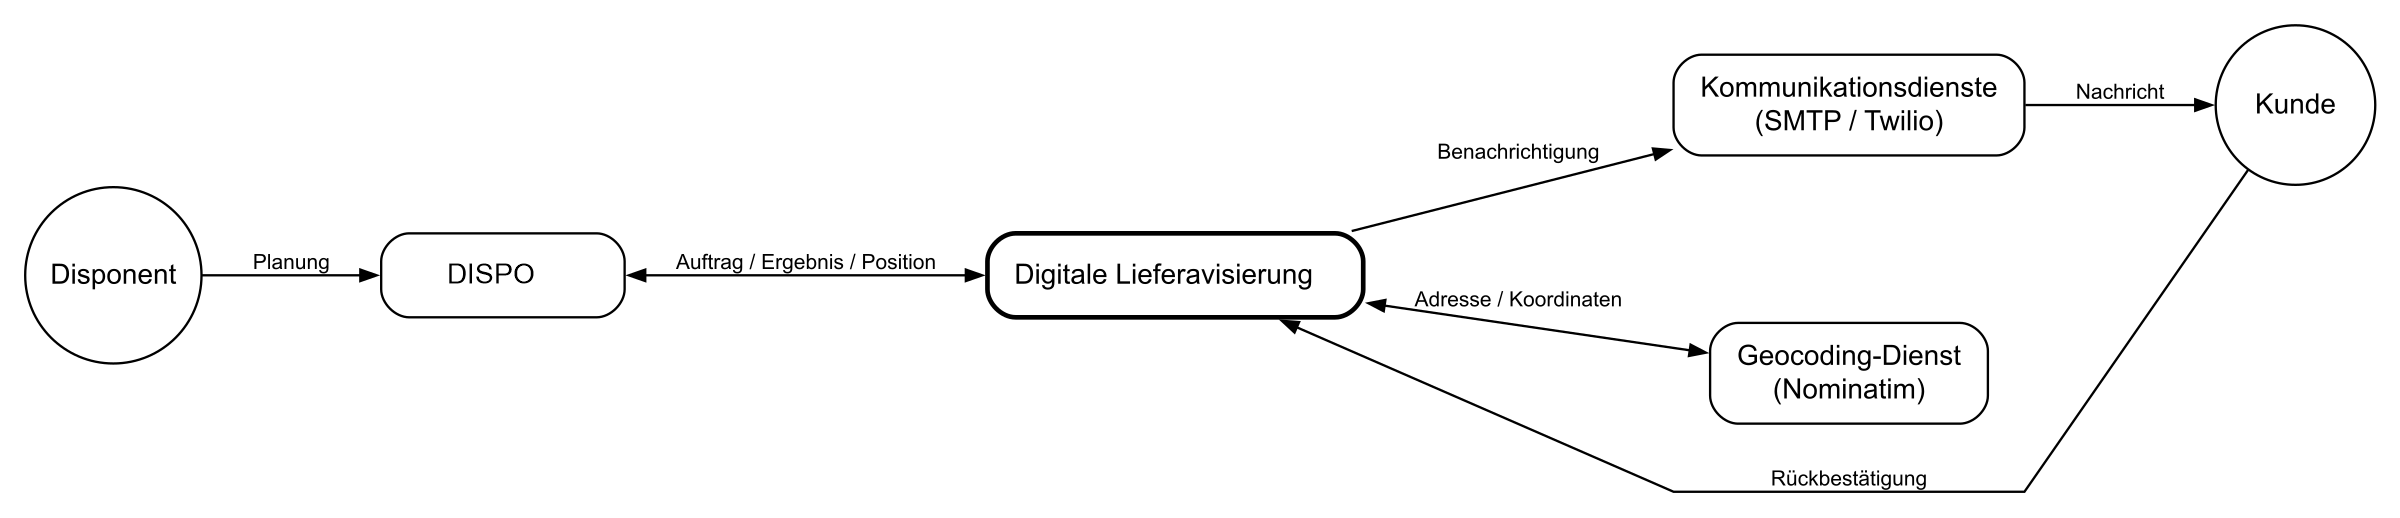
\includegraphics[
    width=\textwidth,
    keepaspectratio
  ]{figures/systemkontext.png}
  \caption{Systemkontext der digitalen Lieferavisierung}
  \label{fig:systemkontext-lieferavisierung}
\end{figure}

Damit bildet die digitale Lieferavisierung eine abgegrenzte Integrationslösung
zwischen DISPO, den beteiligten Benutzern und den externen technischen
Diensten.

\subsection{Systemkomponenten und Verantwortlichkeiten}
\label{sec:systemkomponenten-verantwortlichkeiten}

Das Webfrontend übernimmt die Benutzerinteraktion, der Avisierungsservice die
fachliche Verarbeitung und die PostgreSQL-Datenbank die dauerhafte Datenhaltung.
Der Avisierungsservice bildet das Backend der digitalen Lieferavisierung,
während das Webfrontend die Benutzeroberflächen bereitstellt.
Abbildung~\ref{fig:architekturuebersicht-lieferavisierung} zeigt ihre Einordnung
innerhalb der Systemgrenze.

\begin{figure}[htbp]
  \centering
  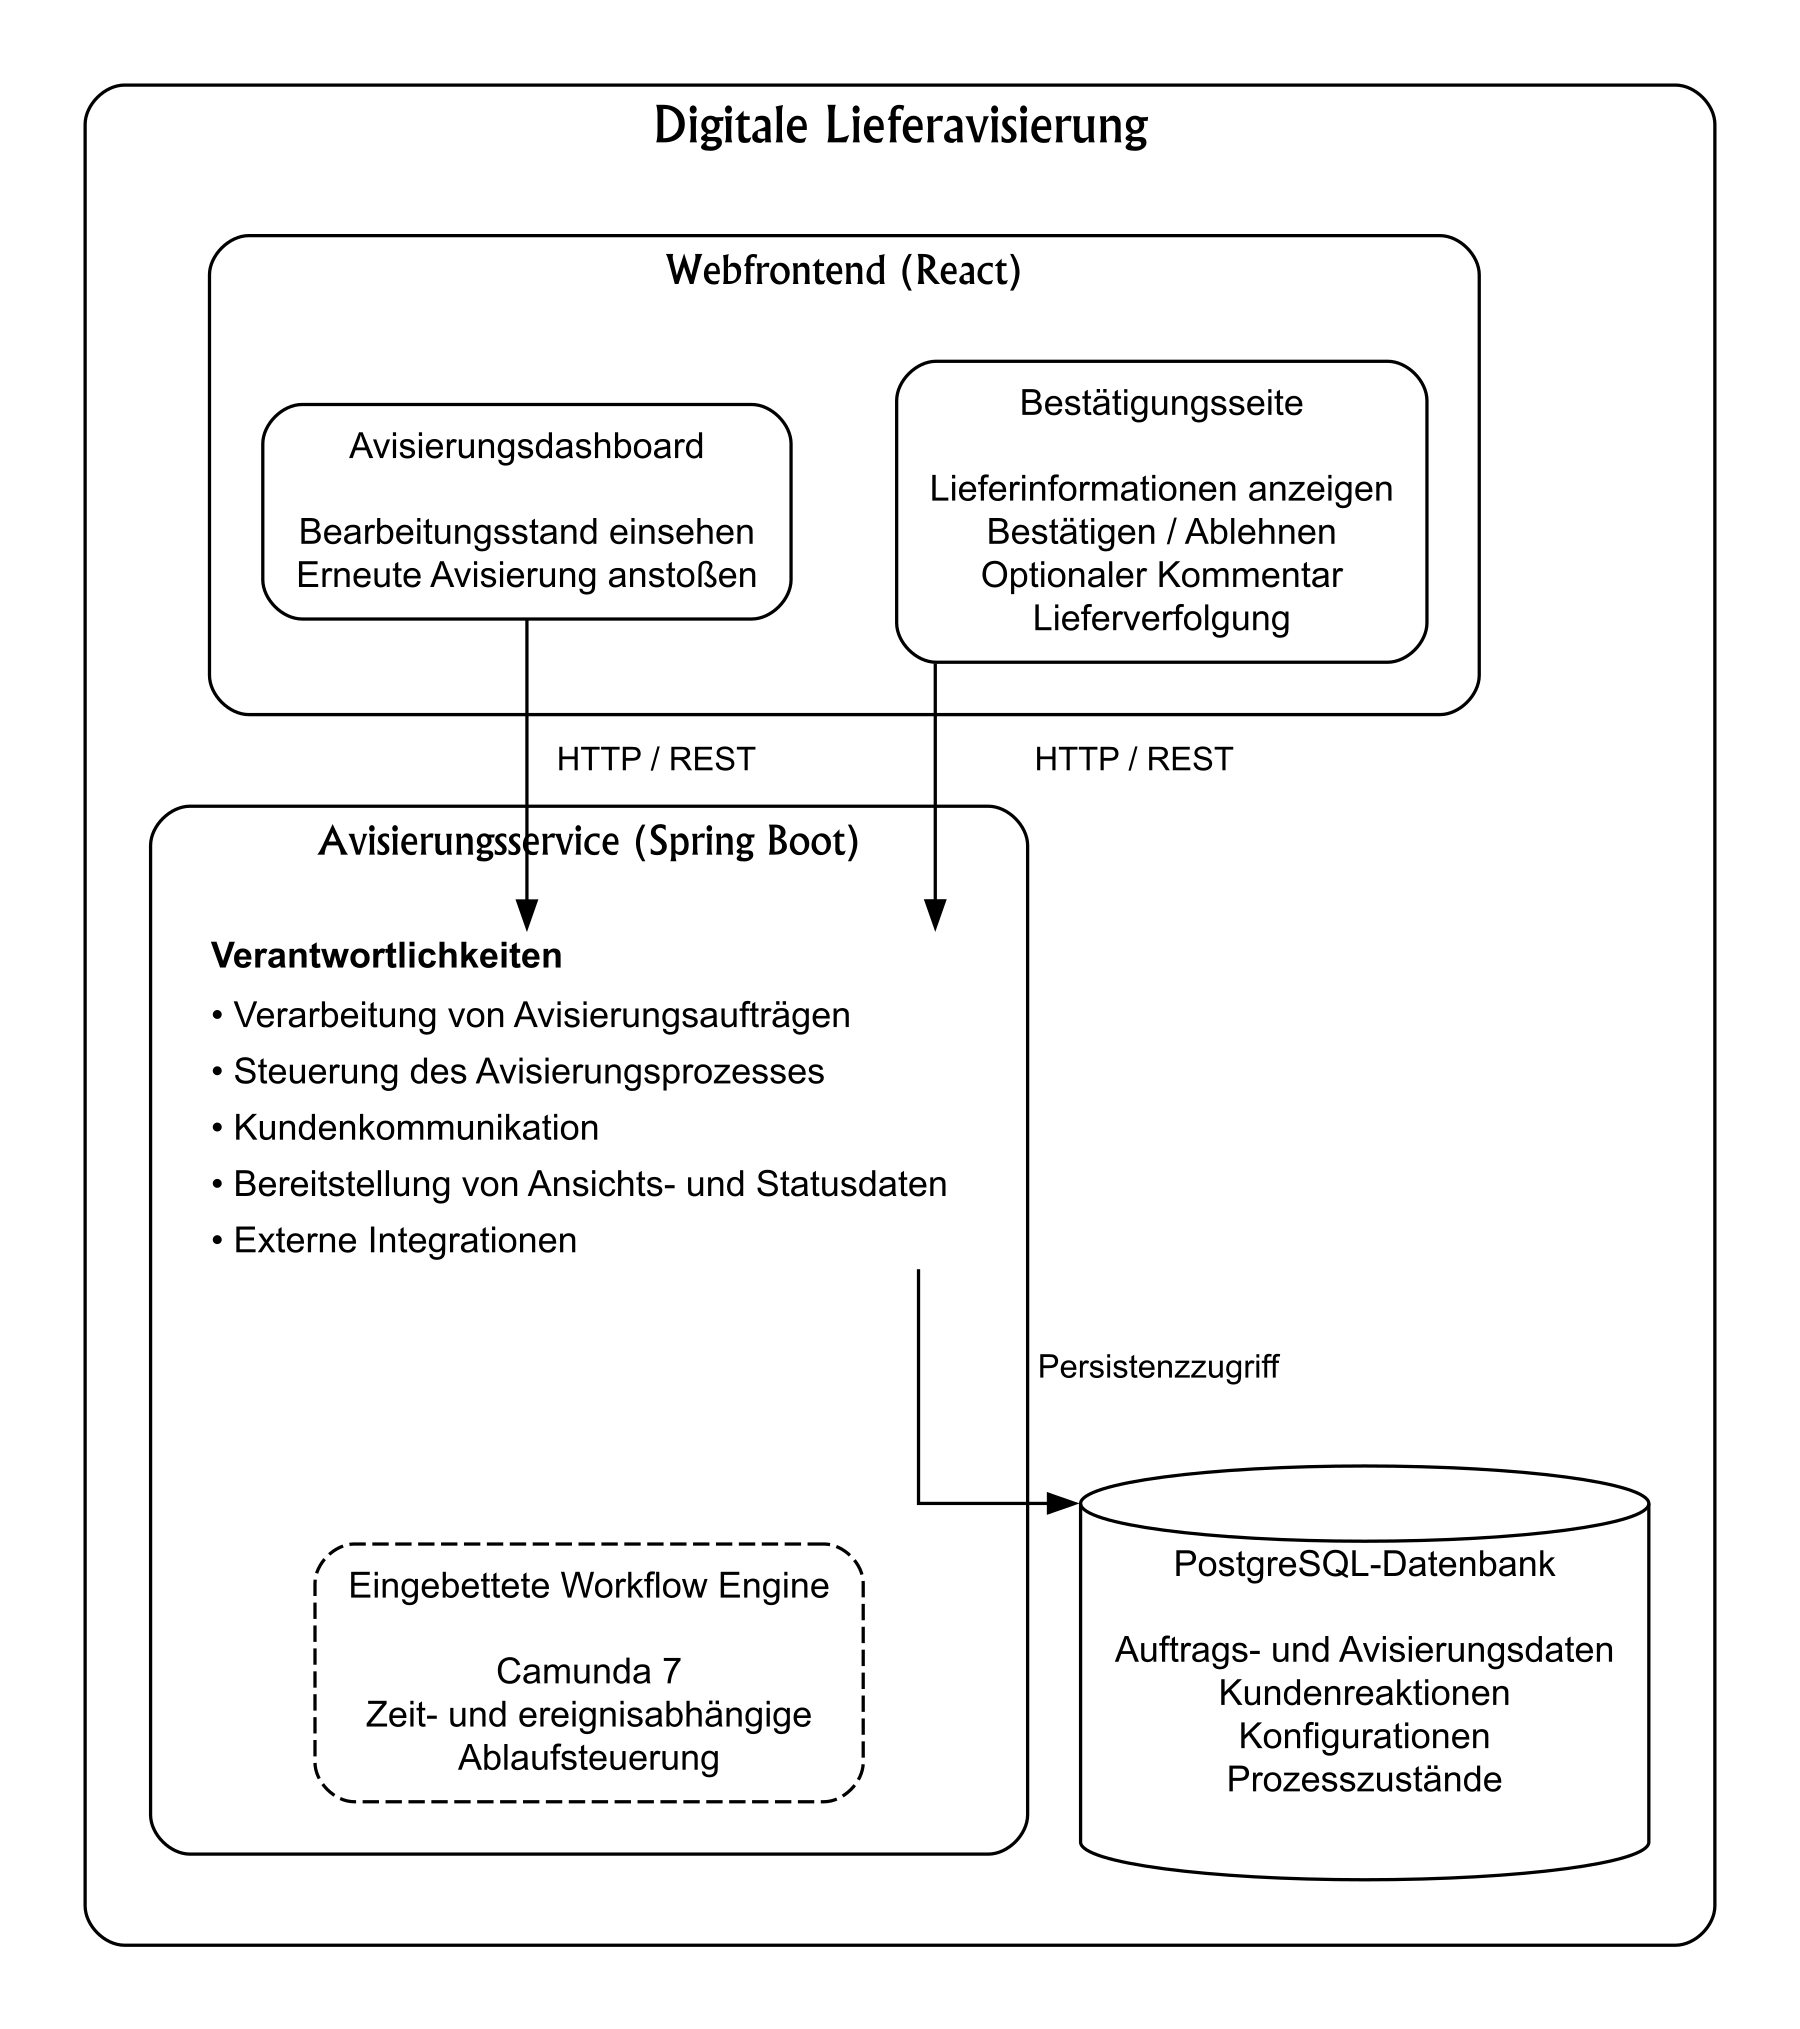
\includegraphics[
    width=0.84\textwidth,
    height=0.72\textheight,
    keepaspectratio
  ]{figures/architekturuebersicht.png}
  \caption{Architekturübersicht der digitalen Lieferavisierung}
  \label{fig:architekturuebersicht-lieferavisierung}
\end{figure}

Das \textbf{Webfrontend} ist als React-Anwendung umgesetzt und umfasst zwei
fachliche Hauptbereiche: das Avisierungsdashboard für den Disponenten sowie
die Bestätigungsseite für den Kunden. Das Avisierungsdashboard zeigt Touren,
Aufträge und Avisierungsstände, ermöglicht das Anstoßen einer erneuten
Avisierung sowie die Verwaltung der mandantenspezifischen
E-Mail-Einstellungen. Über die Bestätigungsseite können Lieferinformationen
eingesehen, Lieferzeitfenster bestätigt oder abgelehnt sowie optionale
Kommentare übermittelt werden. Für bestätigte Vorgänge steht am Liefertag
zusätzlich eine Lieferverfolgung zur Verfügung, sofern die erforderlichen
Positionsdaten verfügbar sind.

Der \textbf{Avisierungsservice} bildet die zentrale fachliche und integrative
Komponente der Lösung. Als Spring-Boot-Anwendung verarbeitet er die aus DISPO
übermittelten Avisierungsaufträge, steuert den Avisierungsprozess, verarbeitet
Kundenreaktionen, koordiniert die Kundenkommunikation und stellt die
benötigten Ansichts- und Statusdaten bereit. Darüber hinaus bindet er externe
technische Dienste an und übermittelt das resultierende Avisierungsergebnis an
DISPO. Die interne Architektur des Avisierungsservice wird in Kapitel 5
vertieft.

Der Avisierungsservice ist mandantenfähig ausgelegt. Auftragsdaten,
Dashboardzugriffe und mandantenspezifische Konfigurationen werden einem
Unternehmen zugeordnet; die konkrete Datenisolation und die zugehörigen
Sicherheitsmechanismen werden in Abschnitt~5.4 erläutert.

Die in den Avisierungsservice eingebettete \textbf{Workflow Engine Camunda 7}
übernimmt die dauerhafte Ablaufkoordination des Avisierungsprozesses. Die
konkrete Workflow-Implementierung wird in Abschnitt 5.2 erläutert.

Die \textbf{PostgreSQL-Datenbank} dient als zentraler Persistenzspeicher
innerhalb der digitalen Lieferavisierung und speichert die für den
Avisierungsprozess benötigten Anwendungs- und Prozessdaten.

\subsection{Schnittstellen und Zusammenspiel der Komponenten}
\label{sec:schnittstellen-zusammenspiel}

Im Folgenden werden die wesentlichen Kommunikationsbeziehungen innerhalb der
digitalen Lieferavisierung sowie zu den angebundenen externen Systemen
betrachtet. Abbildung~\ref{fig:schnittstellenuebersicht-lieferavisierung} zeigt
zunächst die wesentlichen Schnittstellen und Datenflussrichtungen.
Abbildung~\ref{fig:interaktionsablauf-bestaetigung} ergänzt diese statische
Sicht und zeigt exemplarisch das technische Zusammenspiel im
Avisierungsprozess.

\begin{figure}[htbp]
  \centering
  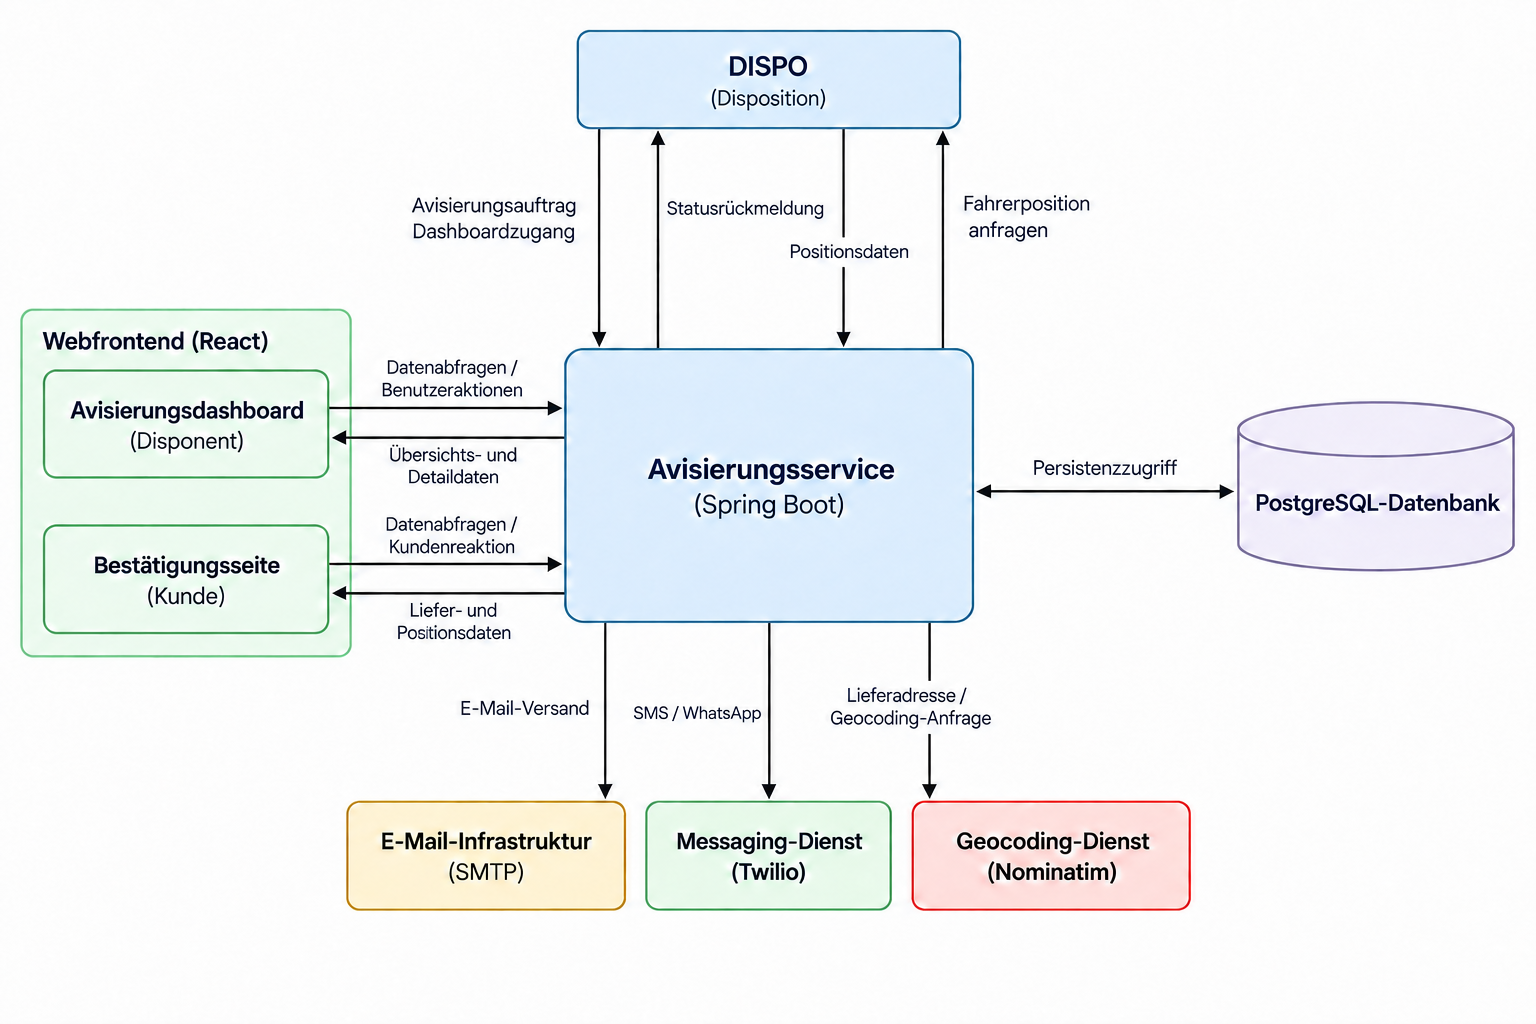
\includegraphics[
    width=\textwidth,
    height=0.68\textheight,
    keepaspectratio
  ]{figures/schnittstellenuebersicht.png}
  \caption{Wesentliche Schnittstellen der digitalen Lieferavisierung}
  \label{fig:schnittstellenuebersicht-lieferavisierung}
\end{figure}

Die Kommunikation mit DISPO umfasst mehrere fachlich unterschiedliche Vorgänge.
DISPO übermittelt Avisierungsaufträge an den Avisierungsservice und initialisiert
bei Bedarf den Zugang zum Avisierungsdashboard. Die spätere Rückmeldung eines
Avisierungsergebnisses erfolgt in Gegenrichtung. Für die
Lieferverfolgung fragt der Avisierungsservice zusätzlich die aktuelle
Fahrzeugposition bei DISPO an und erhält die zugehörigen Positionsdaten zurück.

Auch die beiden Bereiche des Webfrontends kommunizieren direkt mit dem
Avisierungsservice. Das Avisierungsdashboard übermittelt Datenabfragen und
Benutzeraktionen und erhält die benötigten Übersichts- und Detailinformationen
zurück. Der Dashboardzugang wird aus DISPO heraus initiiert; nach dem Übergang
erfolgt die weitere Kommunikation unmittelbar zwischen Webfrontend und
Avisierungsservice. Die Bestätigungsseite wird über den individuellen Link aus
der Kundenbenachrichtigung aufgerufen. Sie bezieht Liefer- und Avisierungsdaten
sowie Daten zur Lieferverfolgung vom Avisierungsservice und übermittelt die
Kundenreaktion an den Avisierungsservice.

Für die Lieferverfolgung werden Daten aus unterschiedlichen Quellen
zusammengeführt. Die Fahrzeugposition stammt aus DISPO, während die geografischen
Koordinaten des Lieferziels über den Geocoding-Dienst ermittelt werden. Hierzu
übermittelt der Avisierungsservice die Lieferadresse als Geocoding-Anfrage und
erhält die bestimmten Zielkoordinaten zurück. Weitere ausgehende Schnittstellen
dienen der Kundenkommunikation: E-Mail-Nachrichten werden über die angebundene
SMTP-Infrastruktur versendet, SMS- und WhatsApp-Nachrichten über den
Messaging-Dienst. Der Zugriff auf die PostgreSQL-Datenbank erfolgt
ausschließlich über den Avisierungsservice und dient der persistenten
Speicherung der für den Prozess benötigten fachlichen und technischen Zustände.

Abbildung~\ref{fig:interaktionsablauf-bestaetigung} zeigt ergänzend das technische Zusammenspiel
innerhalb des Avisierungsprozesses. Die Auftragsübernahme, der Aufruf
der Bestätigungsseite, die Kundenreaktion und die spätere Statusrückmeldung
an DISPO erfolgen zeitlich getrennt. Die Workflow Engine koordiniert diese
zeitlich getrennten Schritte über einen persistent verwalteten Prozesszustand;
die interne
Umsetzung wird in Abschnitt~5.2 erläutert.

\begin{figure}[htbp]
  \centering
  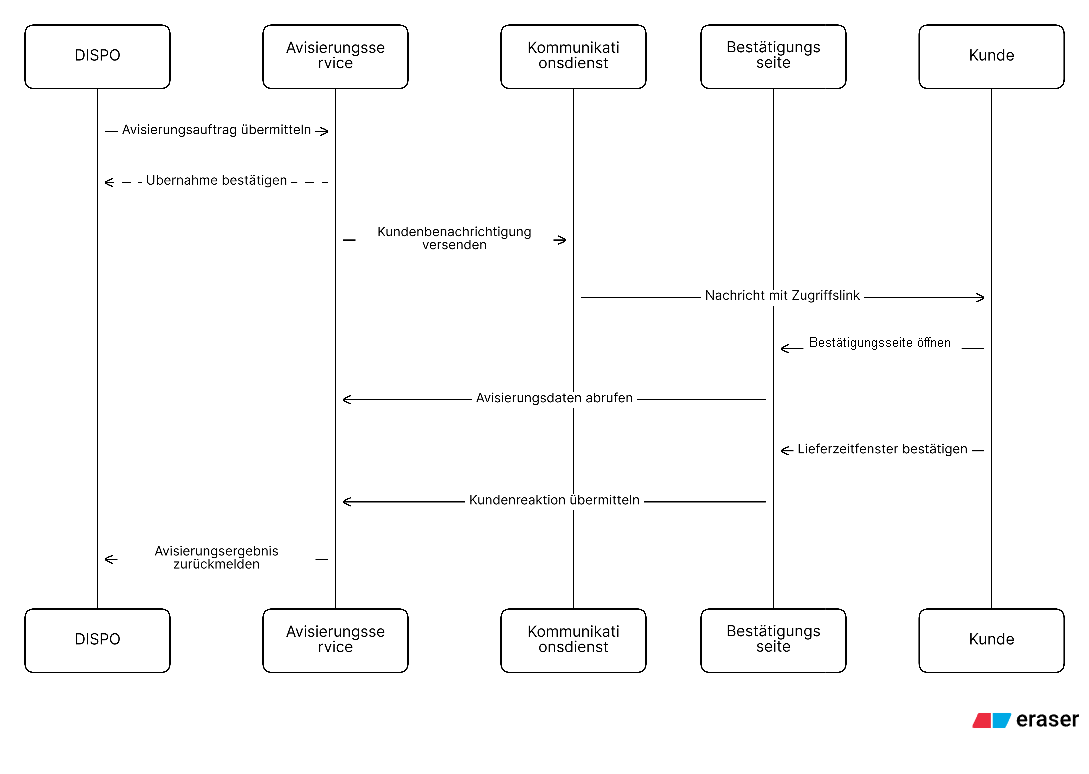
\includegraphics[
    width=\textwidth,
    height=0.70\textheight,
    keepaspectratio
  ]{figures/interaktionsablauf.png}
  \caption{Exemplarischer technischer Interaktionsablauf im Avisierungsprozess}
  \label{fig:interaktionsablauf-bestaetigung}
\end{figure}

\clearpage
